\documentclass[conference]{IEEEtran}
\usepackage{graphicx}
\usepackage{lipsum}
\usepackage{cite}
% *** MATH PACKAGES ***
\usepackage{amsmath}
% *** SPECIALIZED LIST PACKAGES ***
\usepackage{algorithmic}
% *** ALIGNMENT PACKAGES ***
\usepackage{makecell}
\usepackage{array}
\usepackage{float}
\usepackage[utf8x]{inputenc}

\makeatletter
\def\endthebibliography{%
  \def\@noitemerr{\@latex@warning{Empty `thebibliography' environment}}%
  \endlist
}
\makeatother

\author{
    \IEEEauthorblockN{Shashank Reddy Boosi\IEEEauthorrefmark{1}}
    \IEEEauthorblockA{\IEEEauthorrefmark{1} School of Computing\\   { { University of New South Wales}}
    \\\{z5222766\}@student.unsw.edu.au}
}

\begin{document}

\title{Automatic localization of Optic Disc Segmentation using morphological transforms, thresholding and canny detection}


% make the title area
\maketitle

% As a general rule, do not put math, special symbols or citations
% in the abstract
\begin{abstract}

In this paper, I propose a method for localizing optic disc in retinal images. Localizing optic disc s is the key for many segmentation algorithms and disease diagnostics. We use the retinal images to extract the region of interest (ROI) which is the optic disc using morphological operations and then the extracted ROI is used to apply image filtering and thresholding. The Optic disc boundaries is then segmented using Canny edge detection which will separate the Optic disc in the ROI. We experimented the segmentation with different sliding windows and the best metrics is obtained by the 5x5 Morph Ellipse filter with a Jaccard Similarity and Dice Similarity of 65.12\% and 74.15\% respectively.

\paragraph*{Keywords}
Optic Disc, Segmentation, Gaussian Blur, Threshold, Canny, Morphological Transforms.

\end{abstract}

% no keywords



% For peer review papers, you can put extra information on the cover
% page as needed:
% \ifCLASSOPTIONpeerreview
% \begin{center} \bfseries EDICS Category: 3-BBND \end{center}
% \fi
%
% For peerreview papers, this IEEEtran command inserts a page break and
% creates the second title. It will be ignored for other modes.
\IEEEpeerreviewmaketitle



\section{Introduction}
\par

Eye diseases, such as diabetic retinopathy and glaucoma affect the retina and cause blindness which occur in patients with diabetes for more than 5 years. Automated localization of the optic disc (OD) is essential analysis of diabetic retinopathy systems. Accurate localization and detection of optic disc boundary is very useful where fragile vessels develop in the retina. Automatic screening is the key to save many patients by early detection. In this paper, we propose an automated system for optic disk localization and detection. We use Region of Interest(ROI) to extract a region of the optic disc and then apply segmentation and detection algorithms. Once the ROI is extracted we apply the filtering, morphological transforms, in the red channels as red channel has the effect of negating the blood vessels in the optic disc as our goal is only to localize the optic disc and based on which can help to diagnose many eye related diseases.
\par
 The IRRiD data-set \cite{idrid} and the method proposed in this paper are explained from the Section \ref{ssec:describe}. Through the analysis of localizing optic disc, many patients will have early diagnosis of the diabetic retinopathy, glaucoma, fundus diseases.

\section{Background}
\par

Automated system for optic disk localization and detection proposed in \cite{p5}, localizes optic disk using average filter and thresholding, extracts the region of interest (ROI) containing optic disk to save time and detects the optic disk boundary using Hough transform. They mainly used the method for computer analysis of retinal images for diabetic retinopathy and also tested on many different publicly available datasets. They achieved an average accuracy of 96.7\% for localization and an average area under the receiver operating characteristic curve of 0.958 for optic detection.
\par
Another interesting way of localizing optic disc is proposed by \cite{p3} where they present a new template-based methodology for segmenting the OD from digital retinal images. This methodology uses morphological and edge detection techniques followed by the Circular Hough Transform to obtain a
circular OD boundary approximation which was further extended in \cite{p1} where they use optic disc of the four retinal images in DRIVE dataset\cite{drive} to extract the histograms which is used as a kernel. Then, they calculate the average of histograms for each color as template for localizing the center of optic disc which helped them to produce a high success rates of 100, 91.36, and 98.9\%, respectively. Around the same time they was a different proposal \cite{p4} which used watershed segmentation by extracting bright objects from fundus images.
\par
One of the latest research in localization is carried on by  \cite{p2}, where they went with the same approach of using ROI where they claim to reduce the processing area required for optic disc segmentation techniques leading to notable performance enhancement and reducing the amount of the required computational cost for each retinal image. They used the same publicly available datasets like DRIVE\cite{drive} to validate their approach.
\par
This paper is inspired by al of the above related background papers and our method is validated on the IDRiD dataset\cite{idrid} with only 54 images.

\section{Method}                                                                     
Our methodology consists of various steps: Optic Disc Extraction using ROI, Image pre-processing, and Segmentation where we start with preparing the dataset, ROI extraction using Morphological Transform, preprocessing, segmenting. The data-set is taken from IDRiD Grand Challenge \cite{idrid}. We mainly  used opencv for all the steps involved in the methodology. Section \ref{ssec:describe} to section \ref{ssec:metrics} consist of detailed information of the steps.  

\subsection{Data Description}
\label{ssec:describe}
We have a total of 54 retinal and ground truth images for the segmentation method.

\par
The input images contains the 3 channel retinal image and the ground truth is a 1-channel image. Fig \ref{fig:example} shows an example of the IDRiD dataset with retinal and ground truth image.

\par              
\begin{figure}[H]
	\centering
	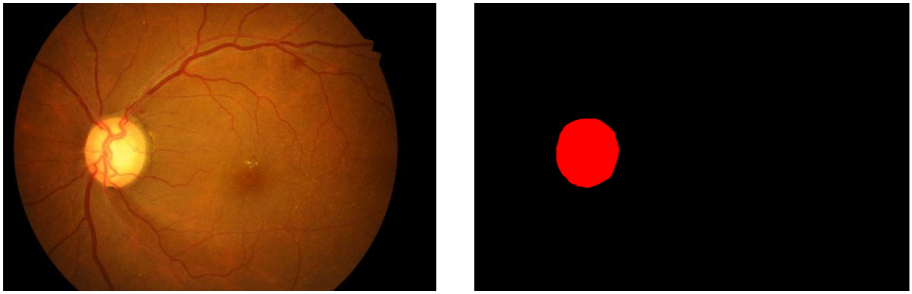
\includegraphics[width=\linewidth]{images/example.PNG}
	\caption{Sample data input and ground truth image}
	\label{fig:example}
\end{figure}

\subsection{ROI Extraction}
\label{ssec:roi}

A series of operations are done of the retinal images to attain an accurate ROI image which comtains the optic disc.

\begin{itemize}
		\item \textbf{Conversion to Gray} The retinal image is converted to a gray image from a BGR image.
		\item \textbf{Blurring} Gaussian blur is then applied to smooth the image and remove any noises that are available in the gray image.
		\item \textbf{Add weighting} We then add weighting by considering the gray image and the noiseless image and the weighting is adjusted to smooth the image over the gray image.
		\item \textbf{Morphological Transformation (Opening)} Morphological transformation of a combination of erosion followed by dilution is applied to clear any bright spots in the retinal image. So that the optic disc could be the one with the highest pixel value. Erosion is done twice and the dilution is done once to remove the bright spots.
		\item \textbf{Histogram Equalization} Histogram equalization is applied after the transforms to spread out the pixel values by having a uniform intensity distribution for the image which will intensify the region of optic disc.
\end{itemize}  

Once all the above operations are done, we calculate the maximum pixel value of the image and consider it a center and extract a 1020x1020 pixel Region of Interest patch image.




\subsection{Image preprocessing}
\label{ssec:preprocess}

Once the Region of Interest is extracted we do the following operations to pre-process the optic disc patch,

\begin{itemize}
		\item \textbf{Red Channel extraction} We split the ROI in to its respective channel and only consider the red channel which will help in negating the blood vessels.
		\item \textbf{Blurring} Gaussian blur is then applied to smooth the image and remove any noises that are available in the red channel.
		\item \textbf{Add weighting} We then add weighting by considering both the image with red channel and the blur image and apply weighting focused on the red channel.
		\item \textbf{Morphological Transformation (Closing)} Morphological transformation of a combination of dilation followed by erosion is applied to clear any spots inside the optic disc so that the segmentation methods can smoothly localize the optic disc. Dilution is done once and the erosion is done thrice to remove the big spots in the optic disc.
\end{itemize}  


\subsection{Image Thresholding}
\label{ssec:threshold}

Preprocessing will make the optic disc white and the region around it to gray as the gray regions inside the optic disc are removed using the closing morphological transform above. We apply the traditional binary thresholding segmentation method and extract the white region of the image. Fig \ref{fig:threshold} shows the ROI patch after thresholding is applied.

\begin{figure}[H]
	\centering
	
\includegraphics[width=150px]{images/threshold.jpg}
	\caption{Image after Threshold segmentation}
	\label{fig:threshold}
\end{figure}

\subsection{Canny Detection}
\label{ssec:canny}

Thresholding gives is the optic disc region and differentiates the optic disc with the whole region and now canny edge detection is used to detect the edge of the segmented optic disc to see if the optic disc is partial or fully localized. Fig \ref{fig:canny} shows the ROI after the canny is applied

\begin{figure}[H]
	\centering
	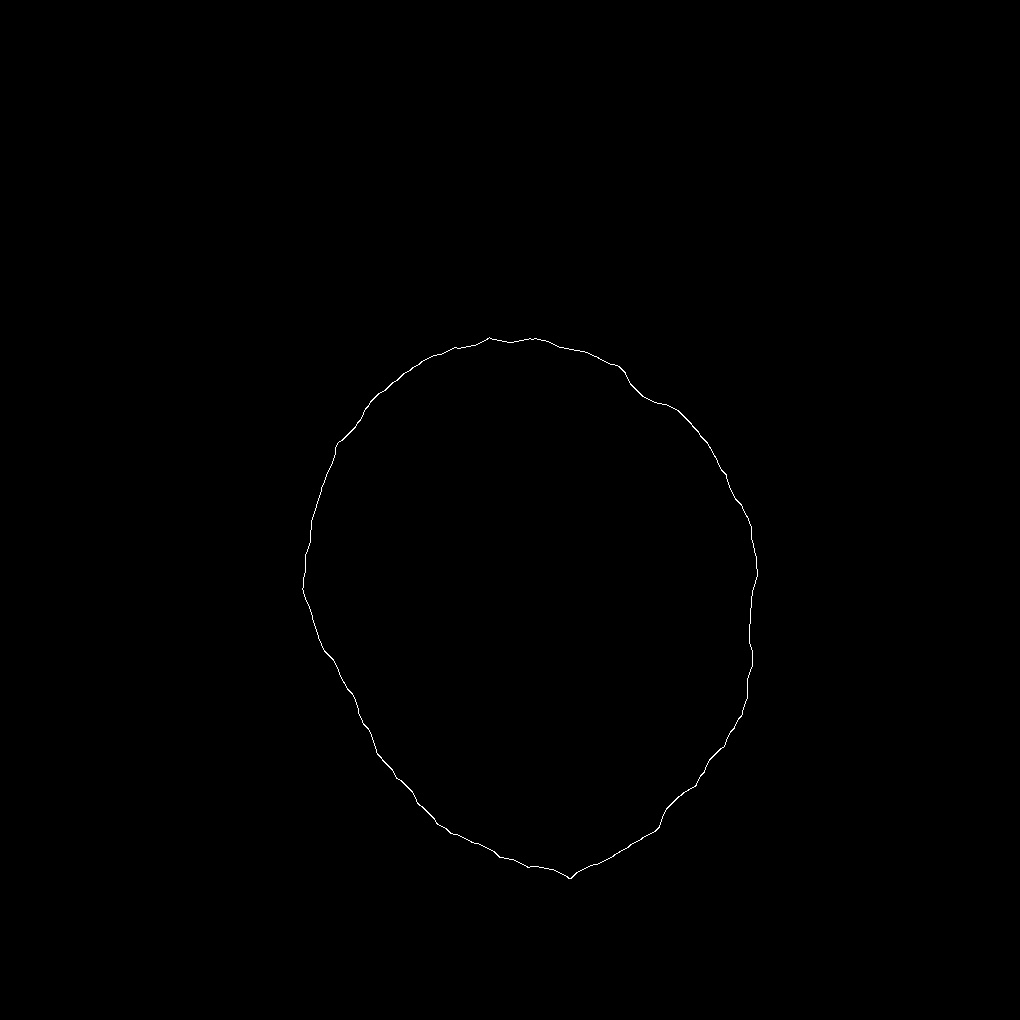
\includegraphics[width=150px]{images/canny.jpg}
	\caption{Image after Canny Edge detection}
	\label{fig:canny}
\end{figure}

\subsection{Metrics}
\label{ssec:metrics}
The combination of all the steps are evaluated under different performance metrics, including Jaccard Similarity Coefficient, Dice Similarity Coefficient for Segmentation. The metrics are defined as following,

\begin{equation}
JSC = \frac{|S \cap T|}{|S \cup T|} = \frac{|TP|}{|TP| + |FP| + |FN|}
\end{equation}

\begin{equation}
DSC = 2\frac{|S \cap T|}{|S| + |T|} = \frac{2|TP|}{2|TP| + |FP| + |FN|}
\end{equation}

where $TP$ is the true positive, $FP$ is the False Positive, $FN$ is the False Negative.

\subsection{Evaluation and Results}
\label{sssec:results}

Table \ref{table:1} shows us the performance in terms of metrics for the method we have experimented. The metrics used for evaluation are Jaccard Similarity, Dice Similarity as shown in the section \ref{ssec:metrics}. Jaccard Similarity and Dice similarity are mainly used for the segmentation of images as the metrics do not include the background while only calculating the intersection over the union. Comparison between other papers is not done because most of the papers use the full dataset if IDRiD and comparing those papers with our implementation would not be correct.As we can see, the comparison between different morphological filter sizes helped us understand the nature of how the segmentation method is acting and predicting based on the metrics. As we can see the lower the filter size the better the performance of the metric. The main reason to get the best Jaccard Similarity score and Dice Similarity score of 65.12\% and 74.15\% is because many images had abnormalities which either contained big lesions which are detected as the optic disc or the brightness around the optic disc is making the method to consider a region that covers the whole brightness.

\begin{table}[H]
\centering
 \begin{tabular}{|c| c c|} 
 \hline
 Morph Filter sizes & Jaccard Similarity & Dice Similarity \\ [0.5ex] 
 \hline
 5x5 & 0.6512 & 0.7415\\ 
 \hline
 10x10 & 0.6348 & 0.7305\\
 \hline
 18x18 & 0.6045 & 0.7102\\
 \hline
 31x31 & 0.5569 & 0.6768\\
 \hline
\end{tabular}
\vspace*{0.25cm}
\caption{Method Performance using different morph filter sizes}
\label{table:1}
\end{table}

Figure \ref{fig:good} and \ref{fig:bad} are the examples for the images with good predictions and the bad predictions. The main difference noticed between the good and the bad predictions is that the images which has a good predictions contains smaller circular spots of lesions which are removed by using morphological transforms but for the bad predictions the lesions are so big and bright that the segmentation model is consider the lesion as the optic disc.

              
\begin{figure}[H]
	\centering
	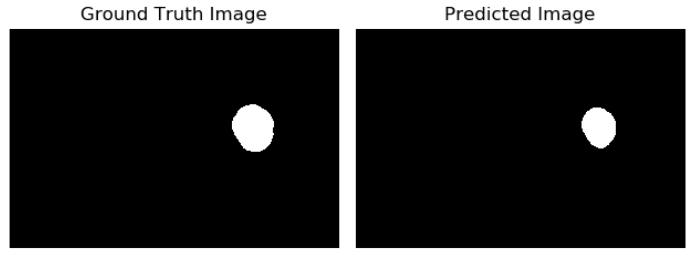
\includegraphics[width=\linewidth]{images/good.PNG}
	\caption{Image with good prediction}
	\label{fig:good}
\end{figure}
  
\begin{figure}[H]
	\centering
	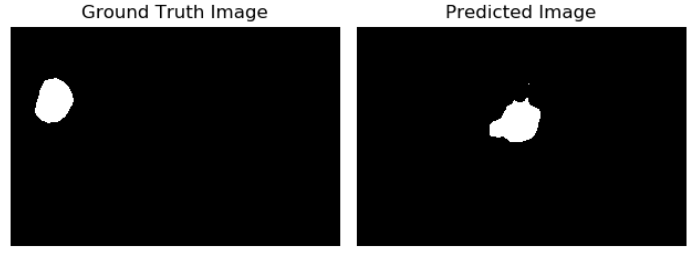
\includegraphics[width=\linewidth]{images/bad.PNG}
	\caption{Image with bad prediction}
	\label{fig:bad}
\end{figure}


\subsection{Conclusion and Future Work}

In this paper, the problem of summarizing a segmentation method for localizing the optic disc on IDRiD datasets is discussed. The focus is mainly on using Region of Interest, Morphological Transform, Red channel filtering to effectively segment the optic disc associated with retinal images \cite{idrid}. The outcome of the predictive results on the IDRiD data-set reveals the Jaccard Similarity Coefficient and Dice Similarity Coefficient with a score of 65.12\% and 74.15\% respectively on a 5x5 morph filter.
\par 
The proposed work can be enhanced by expanding its scope to using Deep Learning and Transfer learning with fully convolutional models like UNet and FCN which will help to accurately find the optic disc but will have to augment the images as Deep Learning feeds off training which needs many examples to become more viable. Another way of enhancing is to use different smoothing operations and segmentation algorithms that is suitable for localization of a region.

\bibliographystyle{IEEEtran}
\bibliography{references}




% that's all folks
\end{document}


